\documentclass[tikz,border=10pt]{standalone}
\usepackage{amsmath,amssymb}
\usepackage{tikz}
\usetikzlibrary{arrows,automata,backgrounds,calendar,chains,decorations,decorations.pathreplacing,decorations.text,fit,matrix,mindmap,patterns,petri,plotmarks,positioning,shadows,shapes,shapes.callouts,shapes.geometric,shapes.misc,spy,trees,calc,intersections,tikzmark,arrows.meta}
\usepackage{xcolor}
\usepackage{pgfplots}
\pgfplotsset{compat=1.16}

% Common math macros from the book
\def\x{\mathbf{x}}
\def\y{\mathbf{y}}
\def\z{\mathbf{z}}
\def\A{\mathbf{A}}
\def\b{\mathbf{b}}
\def\c{\mathbf{c}}
\def\w{\mathbf{w}}
\def\v{\mathbf{v}}
\def\u{\mathbf{u}}
\def\e{\mathbf{e}}
\def\zero{\mathbf{0}}
\def\R{\mathbb{R}}
\def\N{\mathbb{N}}
\def\Z{\mathbb{Z}}
\def\Q{\mathbb{Q}}
\def\st{\text{s.t.}}
\def\vect#1{\mathbf{#1}}
\def\xLP{x^{\mathrm{LP}}}
\def\zLP{z^{\mathrm{LP}}}
\def\xIP{x^{\mathrm{IP}}}

% Common node styles from the book
\tikzset{
    main/.style={circle, draw, fill=gray!20, minimum size=1cm, font=\normalsize},
    dot/.style={circle,fill=blue,minimum size=3pt,inner sep=0pt, outer sep=-1pt},
    vertex/.style={circle,fill=black!25,minimum size=20pt,inner sep=0pt},
    edge/.style={draw,-,thick},
    directed edge/.style={draw,->,>=latex,thick},
}

% Additional macros for 3D/coordinate systems
\newcommand{\xhat}{\hat{\x}}
\newcommand{\yhat}{\hat{\y}}
\newcommand{\zhat}{\hat{\z}}
\newcommand{\ihat}{\hat{\imath}}
\newcommand{\jhat}{\hat{\jmath}}
\newcommand{\khat}{\hat{k}}

\begin{document}
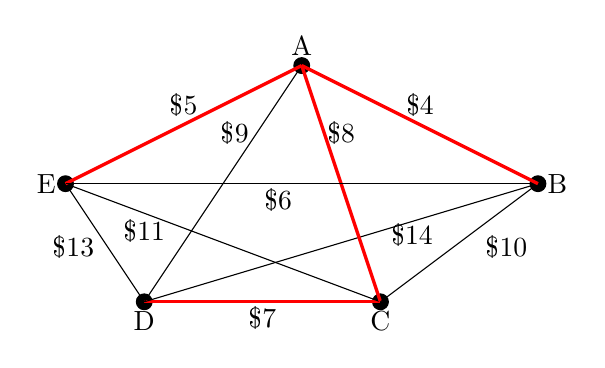
\begin{tikzpicture}
\draw[fill] (0,0) circle[radius=.1] node[below]{D};
\draw[fill] (3,0) circle[radius=.1] node[below]{C};
\draw[fill] (-1,1.5) circle[radius=.1] node[left]{E};
\draw[fill] (2,3) circle[radius=.1] node[above]{A};
\draw[fill] (5,1.5) circle[radius=.1] node[right]{B};
\draw[very thick, red](0,0)--(3,0);
\draw(0,0)--(2,3);
\draw(0,0)--(-1,1.5);
\draw(0,0)--(5,1.5);
\draw(3,0)--(-1,1.5);
\draw[very thick, red](3,0)--(2,3);
\draw(3,0)--(5,1.5);
\draw[very thick, red](-1,1.5)--(2,3);
\draw(-1,1.5)--(5,1.5);
\draw[very thick, red](2,3)--(5,1.5);
\node at (1.5, -0.2){\$7};
\node at (-0.9, 0.7){\$13};
\node at (4.6,0.7){\$10};
\node at (3.5, 2.5){\$4};
\node at (0.5,2.5){\$5};
\node at (1.7,1.3){\$6};
\node at (1.15,2.15){\$9};
\node at (2.5,2.15){\$8};
\node at (0,0.9){\$11};
\node at (3.4,0.85){\$14};
\end{tikzpicture}
\end{document}
